%; whizzy chapter
% -initex iniptex -latex platex -format platex -bibtex jbibtex -fmt fmt
% 以上 whizzytex を使用する場合の設定。

%     Tokyo Debian Meeting resources
%     Copyright (C) 2011 Junichi Uekawa
%     Copyright (C) 2011 Nobuhiro Iwamatsu

%     This program is free software; you can redistribute it and/or modify
%     it under the terms of the GNU General Public License as published by
%     the Free Software Foundation; either version 2 of the License, or
%     (at your option) any later version.

%     This program is distributed in the hope that it will be useful,
%     but WITHOUT ANY WARRANTY; without even the implied warranty of
%     MERCHANTABILITY or FITNESS FOR A PARTICULAR PURPOSE.  See the
%     GNU General Public License for more details.

%     You should have received a copy of the GNU General Public License
%     along with this program; if not, write to the Free Software
%     Foundation, Inc., 51 Franklin St, Fifth Floor, Boston, MA  02110-1301 USA

%  preview (shell-command (concat "evince " (replace-regexp-in-string "tex$" "pdf"(buffer-file-name)) "&"))
% 画像ファイルを処理するためにはebbを利用してboundingboxを作成。
%(shell-command "cd image201101; ebb *.png")

%%ここからヘッダ開始。

\documentclass[mingoth,a4paper]{jsarticle}
\usepackage{monthlyreport}

% 日付を定義する、毎月変わります。
\newcommand{\debmtgyear}{2011}
\newcommand{\debmtgmonth}{8}
\newcommand{\debmtgdate}{20}
% (+ (* (- 2011 2005) 12) 8 -1) started from zero
\newcommand{\debmtgnumber}{79}

\begin{document}

\begin{titlepage}
\thispagestyle{empty}
% タイトルページ:編集必要な部分は最初のマクロに飛ばすこと

\vspace*{-2cm}
第\debmtgnumber{}回 東京エリア Debian 勉強会資料\\
\hspace*{-2cm}
\includegraphics[width=210mm]{image201003/debsen.eps}\\
\hfill{}\debmtgyear{}年\debmtgmonth{}月\debmtgdate{}日

% ここはアップデートすること
\rotatebox{10}{\fontsize{32}{32} {\gt 特集1: XXXX}}

\rotatebox{10}{\fontsize{32}{32} {\gt 特集2: YYYY}}

\vspace*{-2cm}
\hfill{}
\includegraphics[height=6cm]{image200502/openlogo-nd.eps}
\end{titlepage}

\dancersection{Introduction}{上川 純一}

\begin{multicols}{2}
 

 今月のDebian勉強会へようこそ。これからDebianの世界にあしを踏み入れると
 いう方も、すでにどっぷりとつかっているという方も、月に一回Debianについ
 て語りませんか?

 Debian勉強会の目的は下記です。

 \begin{itemize}
 \item \underline{Debian Developer} (開発者)の育成。
 \item 日本語での「\underline{開発に関する情報}」を整理してまとめ、アップデートする。
 \item \underline{場}の提供。
 \begin{itemize}
  \item 普段ばらばらな場所にいる人々が face-to-face で出会える場を提供
	する。
  \item Debian のためになることを語る場を提供する。
  \item Debianについて語る場を提供する。
 \end{itemize}
 \end{itemize}		

 Debianの勉強会ということで究極的には参加者全員がDebian Packageをがりがり
 と作るスーパーハッカーになった姿を妄想しています。情報の共有・活用を通し
 て Debianの今後の能動的な展開への土台として、「場」としての空間を提供す
 るのが目的です。

\end{multicols}

\newpage

\begin{minipage}[b]{0.2\hsize}
 \definecolor{titleback}{gray}{0.9}
 \colorbox{titleback}{\rotatebox{90}{\fontsize{80}{80} {\gt デビアン勉強会} }}
\end{minipage}
\begin{minipage}[b]{0.8\hsize}
\hrule
\vspace{2mm}
\hrule
\begin{multicols}{2}
\tableofcontents
\end{multicols}
\vspace{2mm}
\hrule
\end{minipage}

\dancersection{事前課題}{岩松 信洋}

今回の事前課題は以下です:

Debianの各種ツール(aptとかdpkgとか固有のもの)について、
\begin{enumerate}
\item このツールの解説が欲しい!
\item これの状況はどうなってる?
\item こんなツールありませんか?(あったらいいのに)
\end{enumerate}
と思っていることがあれば、それをできるだけ多く挙げて下さい。

この課題に対して提出いただいた内容は以下です。
\begin{multicols}{2}
{\small
%; whizzy-master ../debianmeetingresume201108.tex
% 以上の設定をしているため、このファイルで M-x whizzytex すると、
% whizzytexが利用できます

\begin{prework}{ 鈴木崇文 }

aptのリポジトリ作成ってどうやるのでしょうか。
ググったらなんかページが出てきてわかりそうですが、やったことないので書きました。
あと、以前誰かが話していたaptのキャッシュサーバーって最近の動向はどうなのでしょうか。

\end{prework}

\begin{prework}{ キタハラ }

Debian固有のものだと、今のところないですね。
1コマンド(又はGUI操作)でUSBメモリにLive環境を作るツールとか?
(探すとあったりして…、調べていません。)

\end{prework}

\begin{prework}{ やまだ }

今後調べたい(解説歓迎)
\begin{itemize}
\item libapt-pkg-perl/python-aptなどのパッケージデータベースAPI
\item debhelper8(簡単になったが奥行きがさらに増した、ような…)
\item *.d.oなサイトを改良したくなったらどうすればいいか
\end{itemize}

緩募
\begin{itemize}
\item apt-buildの./configureの引数なども即いじれる版
\item apt-get changelog風の入れてないマニュアル等を読むツール
\end{itemize}

\end{prework}

\begin{prework}{ koedoyoshida }

dpkg -i(apt-get installも同様)がエラーになったときの原因追及で困ったことがあったので、そのようなときの調査法を知りたい。
\url{http://www.flcl.org/~takasugi/tdiary-org/?date=20061023}
に同現象があったのでとりあえずワークアラウンドは分かりましたが...

\end{prework}

\begin{prework}{ dictoss(杉本 典充) }

debootstrapのおもしろい使い方ってあるのかなぁ。(amd64上でi386環境が必要、常用環境とテスト環境の分離、くらいしか使ったことないです。)
\end{prework}

\begin{prework}{ 上川純一 }
とくになし。

\end{prework}

\begin{prework}{ Osamu MATSUMOTO }

ユーザーとしては特に困ってないっす。aptitudeでしかできない事ってあるのかわかりません。開発者ツールまだまだ勉強中。
\end{prework}

\begin{prework}{ なかおけいすけ }

\begin{itemize}
\item aptのオプションの解説

apt-get update, upgrade, install, remove, clean 位しか使ってないのでその他のオプションについて

\item 推奨パッケージもインストールしてくれるオプション

これはきっとある

\item apt.confの解説

debianのページを見ていると、時々apt.confを修正してみたいな記述があるけれども、何をやっているのか、何ができるのか、解説が欲しい。

\item apt-getとaptitudeの違い
\end{itemize}

\end{prework}

\begin{prework}{ やまねひでき }

debootstrapでxzがサポートされていると良いのかも。
\end{prework}

\begin{prework}{ 岩松 信洋 }

ぱっとは思いつかないです。
\end{prework}

\begin{prework}{ 吉野(yy\_y\_ja\_jp) }

こんにちは。
\end{prework}

\begin{prework}{ yamamoto }

最近は apt-get autoremove で、既に削除されたパッケージの、依存関係解決のために入れられたパッケージがごっそり削除できますが、apt-get build-dep ホゲホゲで入れられたパッケージも同じようにビルド終了後に消せるといいよね。
\end{prework}

\begin{prework}{ taitioooo }

課題は未定ですが。
debianでkaresansuiが使えるようになるといいですね〜

あ、やればいいのか!
\end{prework}

}
\end{multicols}

\dancersection{最近のDebian関連のミーティング報告}{岩松 信洋}
\subsection{東京エリアDebian勉強会77回目報告}

第77回 東京エリアDebian勉強会 を東京オリンピックセンターで行いました。
今回の参加者はやまださん、野首さん、MOTOHARAさん、hattorinさん、キタハラさん、吉田さん、杉本さん、emasakaさん、なかおさん、松本さん、吉野さん、山本さん、前田さん、野島さん、上川さん、岩松の16名でした。
今回は Debian での文書処理紹介ということで、マニアックではありますが上川さんがXSLTの話を、前田さんがSphinxとDoxygenの話をしました。 Wikiフォーマットみたいなのがたくさんあって、覚えるのめんどくさいなと思った勉強会でした。

\subsection{東京エリアDebian勉強会78回目報告}
第78回 東京エリアDebian勉強会 をボスニア・ヘルツェゴビナで行いました。
現地での参加者はやまねさん、野島さん、岩松で、IRCでたくさんの方が参加されました。
レポートは別途。

% (query-replace-regexp "<.*?>" "")
% (query-replace-regexp "^[	 ]\+" "")



\dancersection{Debian Trivia Quiz}{岩松 信洋}

ところで、みなさん Debian 関連の話題においついていますか?Debian関連の話
題はメーリングリストをよんでいると追跡できます。ただよんでいるだけではは
りあいがないので、理解度のテストをします。特に一人だけでは意味がわからな
いところもあるかも知れません。みんなで一緒に読んでみましょう。

今回の出題範囲は\url{debian-devel-announce@lists.debian.org} や \url{debian-devel@lists.debian.org}に投稿された
内容とDebian Project Newsからです。

\begin{multicols}{2}
 %; whizzy-master ../debianmeetingresume201101.tex
% $B0J>e$N@_Dj$r$7$F$$$k$?$a!"$3$N%U%!%$%k$G(B M-x whizzytex $B$9$k$H!"(Bwhizzytex$B$,MxMQ$G$-$^$9!#(B
%
% $B$A$J$_$K!"%/%$%:$OJL%V%i%s%A$G:n@.$7!"$N$A$K%^!<%8$7$^$9!#5U$K%^!<%8$7(B
% $B$J$$$h$&$K$7$^$7$g$&!#(B
% (shell-command "git checkout quiz-prepare")

\santaku
{alioth.debian.org$B$,(B2$BBf$KJ,$+$l$^$7$?!#$=$N%5!<%PL>$O!)(B}
{vasks.debian.org $B$H(B wagner.debian.org}
{volks.debian.org $B$H(B don.debian.org}
{dennys.debian.org $B$H(B gusto.debian.org}
{A}
{$B$[$+$O%U%!%_%l%9$NL>A0(B}

\santaku
{$B8=:_9T$o$l$F$$$k(BPerl transition $B$N(BPerl$B%P!<%8%g%s$O!)(B}
{5.12}
{5.13}
{5.14}
{A}
{5.14$B$O$^$@(Bexperimental$B$G$9!#(B}

\santaku
{$B%W%i%$%^%j%_%i!<%5!<%P$,?7$7$/DI2C$5$l$?9q$O!)(B}
{$B%A%e%K%8%"(B}
{$BCf9q(B}
{$B%^%@%,%9%+%k(B}
{B}
{$B%A%e%K%8%"$H%^%@%+%9%+%k$O%_%i!<!#%W%i%$%^%j$G$O$J$$!#(B}

\end{multicols}

%------------------------------------------------------------------------------
%間に合わず記事にするのは諦めた
%\dancersection{Debianコマンドマップ - 運用管理からパッケージ開発まで}{やまだ}
%------------------------------------------------------------------------------

%------------------------------------------------------------------------------
\dancersection{パッケージビルド七転八倒 - rulesからgit-buildpackageまで}{やまだ}
%------------------------------------------------------------------------------

\subsection{はじめに}
Debianパッケージを作成しようとして、関連するコマンドの層の厚さに
戸惑ってしまった人はいないでしょうか?本稿はパッケージビルドを
rules ベースから git-buildpackage まで一歩づつ発展させることで、
関わってくるコマンドチェインへの理解を深めようと書いてみました。

ところで、今回の内容は「パッケージビルド方法の紹介・講習」ではなく、

\begin{quote}
\Large{自分の手順を晒し、講評を貰って自分の糧とする}
\end{quote}

というのを目しています。要するに

\begin{quote}
\Large{色々やってこういう手順になった、何かもやもや}
\end{quote}

とコメントしてもらう逆講習セッションとなります。ですので、晒している
手順の中では失敗した過程や引っかかった内容と疑問もそのまま書いています。
毎日の迷路での迷いぶりをぜひお楽しみ下さい。

別の方法でできている人は、別記事で手順をぜひ晒してみて下さい!

\subsection{ビルド0日目}

今回の題材は cocot です。これはターミナル側の対応エンコーディングと
実行コマンドの入出力エンコーディングが一致しない場合に

\begin{commandline}
cocot -t UTF-8 -p EUC-JP program-with-euc-jp-only-support ...
\end{commandline}

のように実行するとUTF-8対応コマンドのように使えるというスグレモノなのですが、
今回の話題とは特に関係ないので紹介はこれくらいにします。

0日目の今日は、まずソースのDebianパッケージ化を行います。

\begin{commandline}
$ cd /d/src/
$ git-clone git://github.com/vmi/cocot # ソースはgit公開のみ
$ cd cocot
$ dh_make -c bsd
For dh_make to find the package name and version, the current directory
needs to be in the format of <package>-<version>. 以下略
\end{commandline}

早速エラーとなりました。これはソースフォルダの形式が

\begin{commandline}
<package>-<version>/
\end{commandline}

とバージョン情報を含むことが期待されているためです。が、git clone の
フォルダにバージョン名をつけて運用するというのはイマイチです。さらに、
これから自分が作りこむ debian/ 以下も git 管理したい訳なので、
上の名前でコピーを作って作業するのもしっくりこない。

なので、フォルダ名と関係なく開発・ビルドできる環境を作るために、
従わずにこうします(しました):

\begin{commandline}
$ dh_make -c bsd -n -p cocot_20100903 # --native --packagename を追加
Type of package: single binary, indep binary, multiple binary,
                 library, kernel module, kernel patch or cdbs?
[s/i/m/l/k/n/b] s <- 今回は cocot 単品なので single binary
...
Done. Please edit the files in the debian/ subdirectory now. cocot
uses a configure script, so you probably don't have to edit the Makefiles.
$
\end{commandline}

そして作られた debian/ フォルダ以下のサンプルファイルを削除・編集します。
最終的に

\begin{commandline}
$ ls debian/
total 44
4 README         4 changelog  4 compat   4 copyright  4 manpages  4 source/
4 README.source  4 cocot.1    4 control  4 docs       4 rules*
\end{commandline}

と整理して、ビルド準備が整いました。

\subsection{ビルド1日目 - はじめの一歩}

それではまずは最もシンプルなビルド形態から。これは Makefile に
なっている debian/rules で binary ターゲットを実行するだけです:

\begin{commandline}
$ fakeroot ./debian/rules binary
dh binary
...
dpkg-deb: building package `cocot' in `../cocot_20100903-1_amd64.deb'.
$ ls -d ../cocot*
 4 ../cocot/  20 ../cocot_20100903-1_amd64.deb
\end{commandline}

バイナリパッケージだけなら、これで終わりです。簡単ですね。
fakerootはパッケージ中のファイル所有者が root になるように
併用されるものです。

しかし、このパッケージはDebian品質にはなっていません。

\begin{itemize}
\item 生成されたバイナリパッケージは署名されていない
\item ソースパッケージは生成すらされていない
\item 構成が Debian Policy に準拠しているか未テスト
\end{itemize}

などの問題があるためです。これらは署名なら gpg、ソースパッケージ
生成なら tar/diff/etc(はさすがに原始的過ぎるので普通は dpkg-source)、
構成テストなら lintian があるわけですが、手動でやっていては面倒なので
一括実行するツールが整備されているわけです。

\subsection{ビルド2日目 - dpkg-buildpackage と lintian}

というわけで、「バイナリのみ、しかも未署名未テスト」の状態を
脱するため、debian/rules の直接実行ではなく、ビルドツールを使った
パッケージビルドに進みます。

使う道具は dpkg-buildpackage です。何はともあれまず実行:

\begin{commandline}
$ dpkg-buildpackage -b # まずは binary-only ビルド
...
dpkg-deb: building package `cocot' in `../cocot_20100903-1_amd64.deb'.
 dpkg-genchanges -b >../cocot_20100903-1_amd64.changes
dpkg-genchanges: binary-only upload - not including any source code
 signfile cocot_20100903-1_amd64.changes
...
$ ls -d ../cocot*
 4 ../cocot/                          20 ../cocot_20100903-1_amd64.deb
 4 ../cocot_20100903-1_amd64.changes
\end{commandline}

今度は deb に加えて changes も生成されました。ちゃんと署名しているのも
確認できますね。changes は主にパッケージリポジトリで deb を管理するために
使われるもので、(バイナリ)アップロードの際は deb と changes をペアで
リポジトリにコピーします。

ちなみに、上では構成テストはされていません。これは dpkg-buildpackage は
パッケージ生成に特化しているためです。

\begin{commandline}
$ lintian ../cocot_20100903-1_amd64.changes
W: cocot: new-package-should-close-itp-bug
\end{commandline}

dpkg-buildpackage を使う場合はこのように別途テストします。出てくる
エラーメッセージはタグ名になっており、-i オプションで詳細解説を
表示させたり、また、lintian.debian.org でも同様に細かく知ることができます。

ただ、何が警告されているかは詳しく書かれていても、直し方の例などがなく、
解釈に悩むこともあります。「よくある失敗と直し方」のような情報を
付けられればと、lintian/l.d.oの表示の横にコメント領域を作りたくなります。

ここまでが、バイナリのみ配布する場合の(最小限の)ビルド手順になります。

\subsection{ビルド3日目 - dpkg-buildpackage と git とソースパッケージ}

さて、ここまでソースパッケージの生成はしていませんでした。
これは今回の設定が

\begin{quote}
\Large{普通の git ツリーで Debian package を作る}
\end{quote}

のため、tarball の場合には存在しない .git/ フォルダの扱いを
考慮する必要があるためです。要は、ソースパッケージから .git
フォルダは外したい訳です。

このあたりの問題を完全に解決し git との親和性を高くするのが
後述の git-buildpackage なのですが、それを使うまでは以下のような方法で
対処していました:

\begin{commandline}
$ git-branch upstream # 素のソース保存用ブランチを作っておく
$ git-checkout master # debian/ コミの自分の開発用ブランチを master にする
$ git-add debian/     # debian/ を追加
$ git-commit -a       #
\end{commandline}

このように素のソースツリーと Debian 化した自分の開発用ツリーで
ブランチを分けた上で、

\begin{commandline}
$ git-archive --prefix=cocot-20100903/ upstream \
| gzip > ../cocot_20100903.orig.tar.gz
\end{commandline}

などとして素のソースツリーのみの orig.tar を生成できます。後は

\begin{commandline}
$ dpkg-buildpackage -S # ソースパッケージのみビルド
...
dpkg-source: info: building cocot using existing ./cocot_20100903.orig.tar.gz
dpkg-source: info: building cocot in cocot_20100903-1.debian.tar.gz
dpkg-source: info: building cocot in cocot_20100903-1.dsc
 signfile cocot_20100903-1.dsc
 ...
 signfile cocot_20100903-1_source.changes

$ ls -d ../cocot*
  4 ../cocot/                            4 ../cocot_20100903-1_source.changes
  4 ../cocot_20100903-1.debian.tar.gz  216 ../cocot_20100903.orig.tar.gz
  4 ../cocot_20100903-1.dsc
\end{commandline}

で完成します。署名もされていますね。ちなみに、テストもできます:

\begin{commandline}
$ lintian ../cocot_20100903-1_source.changes
$
\end{commandline}

意味があるかは不明ですが・・・。

とにかく、これでソースパッケージも生成できるようになったので、

\begin{commandline}
$ git-archive --prefix=cocot-20100903/ upstream \
| gzip > ../cocot_20100903.orig.tar.gz
$ dpkg-buildpackage  # 無指定なので dpkg-buildpackage -b -S の両方する
\end{commandline}

でようやくdebian.orgに出せるようなまっとうなパッケージビルドに
届いたことになります。

\subsection{ビルド4日目 - debuildの存在意義に疑問を持つ}

ここまで ./debian/rules、dpkg-buildpackage とビルド方法を
経てきましたが、次はその更に上位のコマンドとなる debuild を
使ってみます。

debuildのdpkg-buildpackageに対する優位性は

\begin{itemize}
\item コマンド名が短くて楽
\item lintianも実行してくれるので楽
\item 署名に debsign や debrsign を使うことができ、柔軟
\begin{itemize}
\item 例:\~{}/.gnupg/ のある生活環境と、パッケージビルドする作業環境が別サーバなど
\end{itemize}
\end{itemize}

というあたりだと思われます。

\begin{quote}
\Large{コマンドチェインを長くする程の価値があるか、微妙}
\end{quote}

という感想を捨てきれませんが、この更に上位のコマンド群は debuild を
呼ぶので、地位は安泰と思われます。

何はともあれ実行:

\begin{commandline}
$ git-archive --prefix=cocot-20100903/ upstream \
| gzip > ../cocot_20100903.orig.tar.gz
$ debuild
...
dpkg-source: info: building cocot using existing ./cocot_20100903.orig.tar.gz
dpkg-source: info: building cocot in cocot_20100903-1.debian.tar.gz
dpkg-source: info: building cocot in cocot_20100903-1.dsc
...
dpkg-deb: building package `cocot' in `../cocot_20100903-1_amd64.deb'.
 dpkg-genchanges  >../cocot_20100903-1_amd64.changes
...
Now running lintian...
W: cocot: new-package-should-close-itp-bug
Finished running lintian.
Now signing changes and any dsc files...
 signfile cocot_20100903-1.dsc Taisuke Yamada <tai@rakugaki.org>
 ...
 signfile cocot_20100903-1_amd64.changes Taisuke Yamada <tai@rakugaki.org>
...
Successfully signed dsc and changes files
$
\end{commandline}

たしかに dpkg-buildpackage よりは少し楽ではあるのですが・・・

\subsection{ビルド5日目 - git-buildpackage - git と Debian の幸せな結婚}

さて、いよいよ git-buildpackage にまでやってきました。これまでは

\begin{commandline}
$ git-archive --prefix=cocot-20100903/ upstream \
| gzip > ../cocot_20100903.orig.tar.gz
$ debuild
\end{commandline}

のように orig.tar は自分で用意してから debuild などを呼んで
いたのですが、git-buildpackage はこの手順を統合します。

\begin{itemize}
\item ブランチAは素のソース管理用で、これを元に orig.tar を生成できる
\item ブランチBはDebian化されたツリーで、これを使ってビルドする
\end{itemize}

という構成を理解して処理してくれる形です。この他にもビルド完了時に
タグを打ってくれたり(--git-tag)、細かい機能が色々あります。

何はともあれ実行:

\begin{commandline}
$ git-buildpackage --git-upstream-branch=upstream --git-debian-branch=master
...
cocot_20100903.orig.tar.gz does not exist, creating from 'upstream'
 dpkg-buildpackage -rfakeroot -D -us -uc -i -I
 ...
$ ls -d ../cocot*
  4 ../cocot/                            4 ../cocot_20100903-1_amd64.changes
  8 ../cocot_20100903-1.debian.tar.gz   20 ../cocot_20100903-1_amd64.deb
  4 ../cocot_20100903-1.dsc            208 ../cocot_20100903.orig.tar.gz
 12 ../cocot_20100903-1_amd64.build
\end{commandline}

キタ!以降は dpkg-buildpackage を呼んでいる通り、これまでと同じです。

で、上では引数を長々と書いていますが、使うブランチ名がデフォルトで
upstream/masterなので、そのようにgitリポジトリを運用していれば

\begin{commandline}
$ git-buildpackage
\end{commandline}

のみでビルド完了になります。

\subsection{ビルド6日目 - pbuilder - えっ、私のビルド、・・・動かない?}

ここまで各種ビルド方法をやってきて、git-buildpackage で一里塚に
到達した感がありますが、

\begin{quote}
\Large{そのパッケージ、本当に他の環境で使えますか?}
\end{quote}

という点が実はまだ甘いままです。

\begin{itemize}
\item パッケージメンテナの環境にしかない非互換のライブラリ
\item パッケージメンテナの環境にしかないカスタマイズされたビルドツール
\end{itemize}

こういったものに依存するバイナリやビルドプロセスが残っていると、
折角アップロードしたパッケージもただのゴミファイルになってしまいます。

これをクリアするためのツールが pbuilder です。これは

\begin{itemize}
\item 独立した deboostrap 環境を作り、
\item その中にパッケージファイルをコピーして、
\item 最後に chroot してビルド
\end{itemize}

をすることで、パッケージメンテナの環境に依存するビルドミスを撲滅します。

まずは実行:

\begin{commandline}
# まずは普通にgit-buildpackageでビルド
$ git-buildpackage
$ ls -d ../cocot*
  4 ../cocot/                            4 ../cocot_20100903-1_amd64.changes
  8 ../cocot_20100903-1.debian.tar.gz   20 ../cocot_20100903-1_amd64.deb
  4 ../cocot_20100903-1.dsc            208 ../cocot_20100903.orig.tar.gz
 12 ../cocot_20100903-1_amd64.build

# 完成物をpbuilder環境内でリビルド。chrootが絡むのでroot権限が必要
$ sudo pbuilder --create # 初回のみ行う(中でdebootstrapする)
$ sudo pbuilder --update # 次回からは更新の上、処理に入る
$ sudo pbuilder --build ../cocot_20100903-1.dsc
...
I: extracting base tarball [/var/cache/pbuilder/sid-amd64/base.tgz]
...
I: Copying source file
I: copying [../cocot_20100903-1.dsc]
I: copying [../cocot_20100903.orig.tar.gz]
I: copying [../cocot_20100903-1.debian.tar.gz]
...
dpkg-source: info: building cocot using existing ./cocot_20100903.orig.tar.gz
dpkg-source: info: building cocot in cocot_20100903-1.debian.tar.gz
dpkg-source: info: building cocot in cocot_20100903-1.dsc
...
dpkg-deb: building package `cocot' in `../cocot_20100903-1_amd64.deb'.
 dpkg-genchanges  >../cocot_20100903-1_amd64.changes
...
\end{commandline}

このように、chroot環境内でリビルドを試みて、ビルドできることの検証と
正しいバイナリの生成を行います。

このようにpbuilderは頑健なパッケージ作成のためにお勧めのツールですが、
いくつか欠点もあります。

\begin{itemize}
\item 大掛かりになるため遅い
\item root権限が必要になる
\item lintian が自動実行されない
\item 署名処理も自動実行されない
\end{itemize}

本質的に解決が難しい部分もあるので、普段はdebuild/git-buildpackageを
使い、最終チェックにpbuilderといった使い分けをしています。また、欠点を
カバーするための上位ツール群も登場しています。

\subsection{ビルド7日目 - pdebuildでダイレクトビルド}

前回は

\begin{itemize}
\item ソースツリーから git-buildpackage が debuild でビルド
\item ビルド結果中のソースパッケージを元に pbuilder がリビルド
\end{itemize}

という2段階実行になっていましたが、考えてみると

\begin{quote}
\Large{それなら最初からchroot環境にソース置いてビルドすれば?}
\end{quote}

という疑問が浮かびます。これを実現するのがpdebuildです。正確には

\begin{quote}
\Large{pdebuild に debuild と同じ CLI I/F を持たせ、入れ替える}
\end{quote}

ことで、git-buildpackage が .git/ の処理をした後で、後は最初から
pdebuild にビルドさせる方式です。pdebuildはオプションでdebsignも
呼び出してくれるので、そこも統合できます。上の方でdebuildの
存在意義に疑問を持っていましたが、このあたりの処理I/Fの基準化という
意味合いもあるのでしょうか?

\begin{commandline}
$ sudo pbuilder --create # 初回のみ行う(中でdebootstrapする)
$ sudo pbuilder --update # 次回からは更新の上、以下続行
$ git-buildpackage --git-builder="pdebuild --buildresult .. --auto-debsign"
...
cocot_20100903.orig.tar.gz does not exist, creating from 'upstream'
...
dpkg-source: info: building cocot using existing ./cocot_20100903.orig.tar.gz
dpkg-source: info: building cocot in cocot_20100903-1.debian.tar.gz
dpkg-source: info: building cocot in cocot_20100903-1.dsc
 dpkg-genchanges -S >../cocot_20100903-1_source.changes
...
I: extracting base tarball [/var/cache/pbuilder/sid-amd64/base.tgz]
...最後にdebsignも呼び出される...
signfile /d/src/cocot_20100903-1.dsc Taisuke Yamada <tai@rakugaki.org>
...
signfile /d/src/cocot_20100903-1_amd64.changes Taisuke Yamada <tai@rakugaki.org>
...
\end{commandline}

再び git ツリーからのパッケージビルドをほぼ一括でやれるようになりました。
ちなみに root 権限が一見不要に見えますがそんなはずもなく、pdebuild は
デフォルトで sudo -E を使って内部で pbuilder を昇格させて処理しています。

なお、Debian Planet 調べでは git-pbuilder なる更に上位のラッパーが
開発途上の模様です。このコマンド階層はどこまで深くなるのか・・・

\subsection{ビルド8日目 - cowbuilder - 高速pbuilderでビルド最終形へ}

前回で git と pbuilder の統合が果たされましたが、pbuilder の
欠点はまだそのまま残っています。この決定を軽減するのが cowbuilder です。

\begin{itemize}
\item ベースの debootstrap 環境を tar.gz で保持せず展開状態で管理する
\item 上記をビルド環境として展開する際、コピーではなくハードリンクを用いる
\begin{itemize}
\item さらに、書き込みはトラップして、ベース環境に書き戻されないよう保護する
\end{itemize}
\end{itemize}

という手法で、処理時間を劇的に短縮します。

\begin{commandline}
$ sudo cowbuilder --create # 初回のみ行う
$ sudo cowbuilder --update # 次回からは更新処理をしてから続行
$ PDEBUILD_PBUILDER=cowbuilder \
git-buildpackage --git-builder="pdebuild --buildresult .. --auto-debsign"
...
dpkg-source: info: building cocot using existing ./cocot_20100903.orig.tar.gz
dpkg-source: info: building cocot in cocot_20100903-1.debian.tar.gz
dpkg-source: info: building cocot in cocot_20100903-1.dsc
 dpkg-genchanges -S >../cocot_20100903-1_source.changes
...
-> Copying COW directory
...以降はpbuilderがchroot/COW環境下でビルドを行う...
\end{commandline}

使い勝手はほとんど同一で

\begin{itemize}
\item pbuilder を使うところを cowbuilder とする
\item pdebuild が cowbuilder を使うよう PDEBUILD\_PBUILDER=cowbuilder と定義する
\end{itemize}

のみで倍速近くになるため、非常に有用です。

この形が、現在のパッケージビルド方法の最終形になるようです。
しかし本稿はまだ続きます。

\subsection{ビルド9日目 - i386 on amd64}

上の git-buildpackage + pdebuild + cowbuilder でビルド手順としては
ようやく完成を見ました。しかし、

\begin{quote}
\Large{ネイティブビルドだけで、いいんですか?}
\end{quote}

という課題があります。

アップロードすればそのうち i386 や他アーキテクチャ用のパッケージも
出来てくる訳ですが、自分で使う自分のパッケージなら、自分でビルドも
してしまいたいものです。アーキテクチャ依存バグを潰すこともできます。

まずは、より簡易な i386 on amd64 ビルドを見てみましょう。
これは gcc レベルでは

\begin{itemize}
\item gcc を gcc -m32 で呼ぶ
\item 依存ライブラリがあれば、それの i386 build 版も用意しておく
\end{itemize}

で済みますが、これをパッケージビルド内でする方法は意外に悩みました。
バイナリがi386なのにパッケージ名がamd64だったり、その逆が起こったり・・・

というわけで、各ビルドツールレベルでの指定方法をまとめてみました:

\begin{commandline}
# debian/rules レベルの場合
CFLAGS=-m32 \
linux32 dpkg-architecture -ai386 -c fakeroot ./debian/rules binary

# dpkg-buildpackage レベルの場合
DEB_CFLAGS_APPEND=-m32 linux32 dpkg-buildpackage -ai386

# debuild レベルの場合
DEB_CFLAGS_APPEND=-m32 linux32 debuild -ai386

# git-buildpackage レベルの場合
git-buildpackage \
--git-builder="DEB_CFLAGS_APPEND=-m32 linux32 debuild -ai386"
\end{commandline}

CFLAGSの指定方法が途中で変わるのは、dpkg-* 系のツールは
ビルドオプションは dpkg-buildflags が供給するものを使うためです。

アーキテクチャ指定については、dpkg-architecture が出力する
DEB\_(BUILD\_HOST)\_* 変数で処理する形が標準で、linux32 の
エミュレーション(uname(3)の結果をいじるだけ)は実質的に意味が
なくなっています。が、お守り代わりでまだ付けたり付けなかったり。

Debian Policyのどこかに

\begin{quote}
\Large{告知:linux32はもうobsoleteです}
\end{quote}

と書いてあったりしないのかな・・・?

\subsection{ビルド10日目 - cross-build on amd64}

今回は ARM や MIPS などのツールチェインがまったく別の場合の
クロスパッケージビルドです。cocot については使う予定は
ないのですが、通信系のツールなどではたまに自分でビルドして
欲しくなります。

実は i386 on amd64 より、まったく別のアーキテクチャ向けの
ビルドをする方が簡単です。

\begin{commandline}
# debian/rules レベルの場合
dpkg-architecture -aarmel -c fakeroot ./debian/rules binary

# dpkg-buildpackage レベルの場合
dpkg-buildpackage -aarmel

# debuild レベルの場合
debuild -aarmel

# git-buildpackage レベルの場合
git-buildpackage --git-builder="debuild -amipsel"
\end{commandline}

当然クロスコンパイラや依存ライブラリのクロス版が入っていることが
前提となりますが、Debianの場合はapt-crossがこのためにあり、容易に
環境を作ることができます。

\subsection{ビルド11日目 - i386 build on amd64 pbuilder}

ここまでのクロスビルドはコンパイラのモード切替やクロスコンパイラで
行っていましたが、pbuilder でもできるのでしょうか?

答は「できる」で、むしろchroot環境でのビルドは、その環境下での
ネイティブビルドとも言えるので更に単純です。ただし、debootstrap の
処理の都合上、こちらは i386/amd64 の方が other/amd64 より楽です。

まずは i386 on amd64 pbuilder から:

\begin{commandline}
$ export DIST=sid ARCH=i386 DISTRIBUTION=sid ARCHITECTURE=i386
$ sudo -E pbuilder --create # 最初の一度だけ行う環境構築
$ sudo -E pbuilder --update # 二回目からは更新だけ行う
$ git-buildpackage --git-builder="pdebuild --buildresult .. --auto-debsign"
\end{commandline}

微妙に DIST=sid ARCH=i386 と DISTRIBUTION=sid ARCHITECTURE=i386 と
同じ事を二重に指定しているのが不審ですが、これは pbuilder と
pdebuild で ARCH/DIST 情報の伝達・参照方法が異なるためです。なお、
マニュアルでは

\begin{commandline}
pbuilder --architecture arch --distribution dist
pdebuild --architecture arch
\end{commandline}

というのがありますが、これは現状あまり有効ではありません(この辺り
もやもやしている)。環境変数の方がコマンドチェインを下っても有効に
なっていやすいので、現在は環境変数べったりに倒してます。

高速化で cowbuilder を組込む場合、pbuilderrc に追加が必要な点のみ
要注意でしたが、ビルド自体は変数設定を1つ増やすだけで済みます:

\begin{commandline}
$ vi /etc/pbuilderrc
...
# for cowbuilder
BASEPATH=/var/cache/pbuilder/$DIST-$ARCH.cow
...
$ export DIST=sid ARCH=i386 DISTRIBUTION=sid ARCHITECTURE=i386
$ sudo -E cowbuilder --create
$ sudo -E cowbuilder --update
$ PDEBUILD_PBUILDER=cowbuilder \
git-buildpackage --git-builder="pdebuild --buildresult .. --auto-debsign"
\end{commandline}

\subsection{ビルド12日目 - cross build on amd64 pbuilder}

だんだん話も終わりに近づいてきました。今度はi386ではない
他アーキテクチャのビルドをpbuilder/cowbuilder on amd64で行ってみます。

他アーキテクチャを扱う上で面倒な点は以下の2つです:

\begin{itemize}
\item debootstrapが一発でchroot環境を構築できない
\item chroot環境内のバイナリはamd64環境で直接実行できない
\end{itemize}

これはいずれもchroot環境さえ作れればいいので、一番手っ取り早い方法は
qemu-*-staticエミュレータを使ってdebootstrapしてしまうことです:

\begin{commandline}
$ cd /var/cache/pbuilder/
$ sudo debootstrap --variant=buildd --include=apt,cowdancer \
--foreign --arch armel sid sid-armel.cow http://localhost:9999/debian
...
$ sudo cp /usr/bin/qemu-arm-static sid-armel.cow/usr/bin/
$ sudo chroot sid-armel.cow /debootstrap/debootstrap --second-stage
...
I: Base system installed successfully.

# 上の --second-stage 実行でクリアされてしまうsources.listを再補充
$ sudo tee sid-armel.cow/etc/apt/sources.list.d/local.list
deb http://127.0.0.1:9999/debian sid main
^D
$ sudo chroot sid-armel.cow apt-get update
\end{commandline}

これは欠点として pbuilder/cowbuilder --create で作った環境ほど
パッケージ構成が最適化されていないようですが、これで

\begin{commandline}
$ export DIST=sid ARCH=armel DISTRIBUTION=sid ARCHITECTURE=armel
$ sudo -E cowbuilder --create
$ sudo -E cowbuilder --update
$ PDEBUILD_PBUILDER=cowbuilder \
git-buildpackage --git-builder="pdebuild --buildresult .. --auto-debsign"
\end{commandline}

とアーキテクチャを問わず同一手順でビルドできるようになりました。

もっとも、qemu-user-static は確実に動作するとは限らないので、
アーキテクチャによって動くような、動かないようなという面は
あります(MIPSですら実は動かないことも…)。

もし cowbuilder ではなく pbuilder で実行する必要があるならば、
単に tarball にして sid-armel/base.tgz に置けば転用できます:

\begin{commandline}
$ sudo mkdir sid-armel
$ cd sid-armel.cow
$ sudo tar zcf ../sid-armel/base.tgz *
\end{commandline}

なお、http://localhost:9999/debian/ は approx で立てている
キャッシングプロキシですが、設定が簡便なのと効果絶大なためオススメです。

\subsection{ビルド13日目 - cross build on amd64 pbuilder, better}

前回は他アーキテクチャ用の chroot 環境を手動 debootstrap で作りましたが、
pbuilder/cowbuilder の生成する環境とは差が出てしまうため、やはり通常の

\begin{commandline}
pbuilder/cowbuilder --create
\end{commandline}

で生成したい所です。そこで、クロス環境もコマンド一回で構築できる
debootstrap-crossを用意して、

\begin{commandline}
pbuilder/cowbuilder --create --debootstrap /usr/local/bin/debootstrap-cross
\end{commandline}

と呼び出してみましょう。スクリプトは単純で、以下の通りです:

\begin{commandline}
#!/bin/sh

archfix() {
  case "$1" in
  armel) echo arm;;
  amd64) echo x86_64;;
  *)     echo $1;;
  esac
}

scanarg() {
  while [ $# -gt 0 ]; do
  case "$1" in
  --arch=)
    ARCH=${$1##--arch=};;
  unstable|testing|stable|oldstable|sid|wheezy|squeeze|lenny)
    set -- "$@"; SUITE=$1; TARGET=$2; MIRROR=$3; SCRIPT=$4; break;;
  esac
  shift
  done

  : ${ARCH:=$(dpkg-architecture -qDEB_HOST_ARCH)}
  : ${SUITE:=sid}
  : ${TARGET:=.}
  : ${MIRROR:=http://127.0.0.1:9999/debian}
}

scanarg "$@"

if dpkg-architecture -e$ARCH; then
  debootstrap "$@"
elif dpkg-architecture -eamd64 && [ $ARCH = i386 ]; then
  debootstrap "$@"
else
  debootstrap --foreign "$@"
  cp "/usr/bin/qemu-$(archfix $ARCH)-static" "$TARGET/usr/bin/"
  chroot "$TARGET" /debootstrap/debootstrap --second-stage
  #echo $MIRROR > "$TARGET/etc/apt/sources.list.d/local.list"
  #chroot "$TARGET" apt-get update
fi
\end{commandline}

これはamd64上でamd64/i386環境を構築するケースも
2段インストールしない本来の形で処理できるので、/etc/pbuilderrc に

\begin{commandline}
DEBOOTSTRAP=/usr/local/bin/debootstrap-cross
\end{commandline}

と書くことで、再び手順は

\begin{commandline}
$ vi /etc/pbuilderrc
...
# for cowbuilder
BASEPATH=/var/cache/pbuilder/$DIST-$ARCH.cow
DEBOOTSTRAP=/usr/local/bin/debootstrap-cross
...
$ export DIST=sid ARCH=i386 DISTRIBUTION=sid ARCHITECTURE=i386
$ sudo -E cowbuilder --create
$ sudo -E cowbuilder --update
$ PDEBUILD_PBUILDER=cowbuilder \
git-buildpackage --git-builder="pdebuild --buildresult .. --auto-debsign"
$ lintian ../mypackage*.deb
\end{commandline}

とアーキテクチャを問わず同様となります。

\subsection{ビルド14日目 - 大統一ビルドの失敗 - pbuilder に lintian 統合}

ここまで、素の debian/rules ビルドから一歩ずつ進めて、

\begin{quote}
debian/rules
$\rightarrow$ +dpkg-buildpackage
$\rightarrow$ +debuild
$\rightarrow$ +git-buildpackage
$\rightarrow$ +pbuilder
$\rightarrow$ +pdebuild
$\rightarrow$ +cowbuilder
$\rightarrow$ +i386 build support
$\rightarrow$ +generic cross build support
\end{quote}

と1つずつ機能を組み込んできました。しかし、pbuilder 以降はlintianが
統合から外れている事に気付かれているでしょうか?

これには理由がある(と思われる)のですが、組み込み自体は実は可能です。
pbuilder(そしてそれを利用している cowbuilder)にはフック機能があり、
各種処理の前後で任意のスクリプトでフックできます。

実は既に /usr/share/doc/pbuilder/examples/ に用意されているのですが、
これを利用してビルド完了直後に lintian を呼んでみましょう。

\begin{commandline}
$ mkdir /t/pbhook/
$ cp /usr/share/doc/pbuilder/examples/B90lintian /t/pbhook/
$ PDEBUILD_PBUILDER=cowbuilder \
git-buildpackage --git-builder="pdebuild \
--buildresult .. --auto-debsign -- --hookdir /t/pbhook"
...
I: user script /d/cache/pbuilder/build/cow.13001/tmp/hooks/B90lintian starting
...
Get:19 http://127.0.0.1/debian/ sid/main lintian all 2.5.2 [617 kB]
...
Setting up lintian (2.5.2) ...
Generating en_US.UTF-8 locale for internal Lintian use....
+++ lintian output +++
W: cocot: new-package-should-close-itp-bug
...
+++ end of lintian output +++
I: user script /d/cache/pbuilder/build/cow.13001/tmp/hooks/B90lintian finished
...
\end{commandline}

これでビルド+署名+検証を完全実行するビルド手順の大統一が再び果たされました。

・・・が、やってみると判るのですが、ネイティブビルドなら
まだしも、クロスビルドの時にエミュレータ上でlintianを実行するのは
正直遅いです。上の Generating locale ... の辺りでかなりぐんにゃり。

結局、餅は餅屋で

\begin{itemize}
\item テストビルドをネイティブのdebuild環境でやりつつlintianも連動実行
\item 最終的なクリーンビルド・バイナリ生成はpbuilder環境
\item 署名はせずに、アップロードまたは独自リポジトリ設置のタイミングで実行
\end{itemize}

と、むしろ統一しないほうがいい、というのが結論です。

\begin{quote}
\Large{ここまで引っ張っておいてそれが結論か!}
\end{quote}

どうぞ皆様は同じ過ちは犯されませんように・・・

\subsection{まとめ}

今回は debian/rules による単純な(といっても、この中身は debhelper という
別の闇が控えてます・・・)ビルドから始めて、git-buildpackage での git 統合、
さらに pbuilder/cowbuilder でのクリーンビルド、そしてさらにクロスビルドまで
含んでの手順統一を行ってきました。

すべてを勘案した、現在のビルドの最終形はこうなっています:

\begin{commandline}
=== /etc/pbuilderrc ===
...
# for cowbuilder
PDEBUILD_PBUILDER=cowbuilder
if echo $SUDO_COMMAND | grep -q qemubuilder; then
  BASEPATH=/var/cache/pbuilder/$DIST-$ARCH.qemu
else
  BASEPATH=/var/cache/pbuilder/$DIST-$ARCH.cow
fi
  
# このコマンドの内容はビルド13日目を参照
DEBOOTSTRAP=/usr/local/bin/debootstrap-cross
...
\end{commandline}

この設定でマルチアーキテクチャ対応の pbuilder/cowbuilder 環境が
整うので、後は

\begin{commandline}
$ export DIST=sid ARCH=i386 DISTRIBUTION=sid ARCHITECTURE=i386
$ sudo -E cowbuilder --update # たまに行っておく。初回だけ --create になる
$ git-buildpackage --git-builder="pdebuild --buildresult .."
$ lintian ../$(basename $PWD)*.deb
$ debsign ../$(basename $PWD)*.changes ../$(basename $PWD)*.dsc
\end{commandline}

を実行、という形に落ち着いています。

この先には qemubuilder という大物や、アップロード/野良リポジトリ運営との
統合などがテーマとしてまだあるのですが、今日の所はこれくらいで締めさせて
頂きます。それでは

\begin{quote}
\Large{Happy Building!}
\end{quote}

%-------------------------------------------------------------------------------
\dancersection{パッケージを作ったらスポンサーアップロード}{岩松 信洋}
%-------------------------------------------------------------------------------
\label{sec:sponsorupload}
\index{sponsor upload}

\subsection{はじめに}
%* Debian Developers
%* Debian Maintainers (DM)
% Sponsored maintainers

Debian にパッケージをアップロードする場合、誰でもアップロードできるわけではなく
限られた人しかアップロードできません。
アップロードできるのはDebian Developer(以下、DD)とDebian Maintainer(以下、DM)
だけです。また、DM はアップロードする際に制限があります。


%この制限にはパッケージが新しく追加されること、
%
%- 制限を書く

 
DDではない人が、メンテナンスしているパッケージをアップロード
する場合には、DD に頼んでアップロードしてもらう必要があります。
パッケージを代理でアップロードする人をスポンサーといい、アップロードする行為を
スポンサーアップロードといいます。
パッケージメンテナに変わってパッケージをアップロードするので、パッケージに対して
責任が問われる作業です。
よって、アップロードするパッケージの内容やパッケージメンテナについてある程度知
っておく必要があります。
スポンサーはパッケージのチェック等を行ったりパッケージ内容に対して助言をす
るので、mentor(助言する人)といった方がわかりやすいかもしれません。 
このパッケージチェックの過程は DD や DM
になる場合に優位に働く場合があります。DDやDMになる時には既存のDDに支持者になって
もらう必要があるのですが、この場合スポンサーに支持者担ってもらうように依頼すると、
しっかりした内容の支持内容を提供してくれるはずです。

では、スポンサーがどのようにしてパッケージをスポンサーアップロードするのか
説明します。

\begin{figure}[ht]
 \begin{center}
  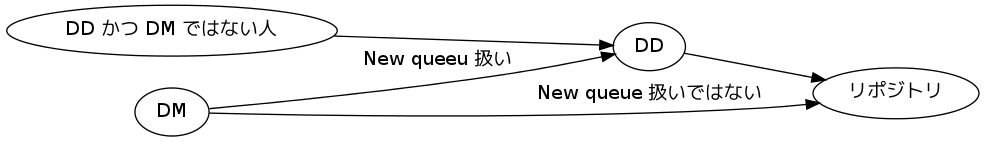
\includegraphics[width=0.8\hsize]{image201108/sponsor0.png}
 \end{center}
\label{fig:sponsor0}\caption{パッケージアップロード}
\end{figure}

\subsection{スポンサーアップロードするときに確認する内容}

パッケージメンテナに「アップロードして!」と言われてはいはいと 
アップロードしてしまうと変なパッケージがDebianのパッケージ
リポジトリに入ることになり、いろいろ問題が起きてしまいます。
よって、スポンサーはアップロードするパッケージメンテナとパッケージを
確認する必要があります。
スポンサーは確認する前と後にチェックする内容があります。スポンサーによって内容が異なりますが、
ここでは私が行っているチェック内容を紹介します。

\subsubsection{パッケージをチェックする前のチェック}

スポンサーをするパッケージメンテナの方に以下の内容を確認しています。

\begin{itemize}
\item Web of Trust(WOT) に入っているか。

GPGの鍵チェックを行います。WOT に入ってない場合には近くにいるDDにキーサインしてもらうように
依頼しています。

\item DDやDMへの意欲はあるか。

ただパッケージメンテナになるのもいいのですが、私を含めたスポンサーの多くは、
メンテナには最終的に DDになってもらって、Debianの開発に参加して欲しいと思っている
と思います。よって、パッケージメンテナの次のステップについて考えているか、確認しています。
私はDDやDMになりたくないからといって、スポンサーにならないことはないです。

\item Debian 新メンテナーガイド\footnote{\url{http://www.debian.org/doc/manuals/maint-guide/}} を読んだか。
\item DFSG \footnote{\url{http://www.debian.org/social_contract.ja.html}} を読んだか。
\item Debian Policy\footnote{\url{http://www.debian.org/doc/debian-policy/}} を読んだか。
\item Debian Reference \footnote{\url{http://www.debian.org/doc/manuals/developers-reference/}}を読んだか。

これらは読んでおくべきドキュメント類です。読んでないと話
にならないので、まず読んである程度理解してもらうようにしています。

\end{itemize}

これ以外にも、たまに誰もスポンサーする人がいないようなのでスポンサーする場合があります。

\subsubsection{パッケージのチェック}

次に実際のパッケージのチェックを行います。
内容は以下になります。

\begin{itemize}

\item ライセンスの確認

ソフトウェアのライセンスがDFSGに合致するライセンスか、
ライセンスが debian/copuright に書かれているか確認します。
この確認には devscripts パッケージに含まれる licensecheck を使うことが多いです。

また、最近ではdebian/copyright のフォーマットには、
DEP5
\footnote{\url{http://dep.debian.net/deps/dep5/}}
に対応しているか確認しています。
仮に不明な場合には上流開発者に問い合わせるようにメンテナにお願いします。

\item orig.tar.gz の確認

オリジナルのtarボールと一緒か、オリジナルのソースコードに
変な改変をしていないかを確認します。

\item 最新のパッケージングのルールに合っているかの確認。

例えば、使っているプログラミング言語向けのパッケージングサポートツールが新しくなっていたり、
パッケージングポリシーが決まっている場合があります。できるだけ新しいパッケージングのルールに
合わせるようにします。

\item debian/control ファイルの確認

依存関係、パッケージの説明、各セクションの確認を行います。

\item debian/rules の確認

シンプルな構成になっているか、ポリシーに違反していないかの確認。

\item pbuilder を使ったパッケージビルドの確認

最新unstable ディストリビューションでパッケージがビルドできるか確認します。
lintian によるチェックや、ビルドに必要なパッケージが依存関係から漏れていないか
確認することができます。
この時に使うツールは pbuilder\footnote{\url{http://packages.qa.debian.org/p/pbuilder.html}}(cowbuilder\footnote{\url{http://packages.qa.debian.org/c/cowdancer.html}})と、
sbuild\footnote{\url{http://packages.qa.debian.org/s/sbuild.html}} です。
手元でビルドしてアップロードする場合には pbuilder を使っています。
スポンサーをしているパッケージは定期的にビルドの確認を行うようにしており、
これには sbuild を使っています。

\item lintianを使ったポリシーとパッケージングミスの確認

パッケージが Debian ポリシー に準拠しているか簡単に確認するには
lintian\footnote{\url{http://packages.qa.debian.org/l/lintian.html}} を使います。
これはDebian ポリシー の他に Debian パッケージのよくある間違いに関してチェックしてくれます。

\item メンテナスクリプト(preinst、postinst、prerm、postrm、コンフィグ)の確認

これらは動くのか、必要なものなのかをチェックします。

\item オリジナルの tar ボールとの差分の確認

diff.gz の内容を確認します。
作成されたパッチは上流開発者に送ってあるか、パッチはDEP3
\footnote{\url{http://dep.debian.net/deps/dep3/}}
に対応しているか、確認します。

\item パッケージのインストール、アンインストール、動作確認

パッケージはできても、インストールできない場合やアンインストールできない場合があります。
またパッケージが動作しない場合もあります。このような問題
がないか確認するために、
piuparts\footnote{\url{http://packages.qa.debian.org/p/piuparts.html}} を使ってインストール、アンインストールのチェックと、実際にインストールしてみて動作するか確認をします。

\end{itemize}

\subsubsection{その他}
その他、スポンサーによっては以下のような理由でスポンサーしてくれない場合があるようです。
注意しましょう。

\begin{itemize}

\item スポンサーをUploaderに入れることを要求される場合がある。

これは、パッケージメンテナの代わりにパッケージをアップロードする場合に有効です。
先に説明したように、パッケージのメンテナンスの責任はスポンサーにもあるのためです。

\item パッケージング用のツールを要求される場合がある。

例えばスポンサーによっては、パッケージにcdbs を使っている場合、debhelper を使うように言われる場合があるようです。

\item \url{http://mentors.debian.net} を使わない場合はスポンサーをしない。

信頼できる以外にアップロードされたソースパッケージは信頼しないというポリシーのようです。

\item 自分の知らないプログラミング言語で書かれたパッケージはスポンサーをしない。

\end{itemize}

また、\url{http://wiki.debian.org/SponsorChecklist}
に実際にスポンサーしている人の方針が纏められています。

\subsection{アップロード}
アップロードには、dput や dupload パッケージを使います。
実装が異なるだけで、基本的な機能は揃っているのでどちらでも使い方は同じです。

\subsection{まとめ}
以上のようにスポンサーになることはとても大変なので、メンテナの方はさっさとDMかDDがになりましょう。

%------------------------------------------------------------------------------
\dancersection{LT: aufsbuilder - cowbuilderにたたかいをいどむ}{やまだ}
%------------------------------------------------------------------------------

\subsection{やってみた}
数年前にaufsがマイブームだった時、
\begin{quote}
\Large{これでaufsbuilder書いたらcowbuilerに勝てるんじゃね?}
\end{quote}
と思ってやってみたものの、僅差ながら負けてお蔵入りしていた
aufsbuilderがこのほど勝利したので報告します。

\subsection{つくりかた}
実は pbuilder は chroot 環境に任意の場所を指定することができ、

\begin{commandline}
pbuilder $PBCMD --no-targz --buildplace <適当なchroot先>
\end{commandline}

と呼び出してやるだけで、よろしくビルドしてくれます。なので、
これを呼び出す前にテンプレート用chroot環境に書き込み用使い捨て
フォルダをラップしたaufs chrootを作ってやればいいわけです。

以下コード:
\begin{commandline}
#!/bin/sh -e

: ${PB_BASE=/var/cache/pbuilder}
: ${PB_WORK=/var/cache/pbuilder/build}

usage() {
  P=$(basename $0)
  test $# -gt 0 && echo $@ >&2
  cat <<EOF 1>&2
$P - pbuilder wrapper with aufs-wrapped chroot
Usage: $P ...pbuilder-args...
Note:
- You need to define PB_BASE and PB_WORK
- For base chroot tree, \$PB_BASE/\$ARCH-\$DIST.cow/ will be used.
- For actual work tree, \$PB_WORK/\$\$/ will be used.
- Default: PB_BASE=$PB_BASE, PB_WORK=$PB_WORK
EOF
  exit 1
}

# pass all args to pbuilder (0 args == help)
test $# -gt 0 || usage
test $# -gt 0 && PBCMD="$1"; shift
test $# -gt 0 && PBARG="$@"

# prepare env
: ${DIST:=sid}
: ${ARCH:=$(dpkg-architecture -qDEB_HOST_ARCH)}
export ARCH DIST

MT="$PB_WORK/$$"
RW="$PB_WORK/$$/rw"
AD="$PB_BASE/$DIST-$ARCH"
RO="$PB_BASE/$DIST-$ARCH.cow"

# sanity check
test -d "$MT" && usage "ERROR: Workdir already exists: $MT"
test -d "$RW" && usage "ERROR: Workdir already exists: $RW"
test -d "$RO" || usage "ERROR: Missing template: $RO"

# register cleanup hook
trap "
$DEBUG umount -lf '$MT/var/cache/apt' '$MT' && $DEBUG rm -fr '$MT'
" 0 1 2 3 4 6 7 8 11 15

# prepare chroot tree
$DEBUG mkdir -p "$RW" "$AD/aptcache"
$DEBUG mount -t aufs -o "br:$RW:$RO=ro" none "$MT"
$DEBUG mount --rbind "$AD/aptcache" "$MT/var/cache/apt"

# run pbuilder
$DEBUG pbuilder $PBCMD --aptcache "" --no-targz --buildplace "$MT" "$@"
\end{commandline}

\subsection{たたかってみる}

pbuilderとcowbuilderの関係同様、aufsbuilderもpbuilder互換なので
そのまま

\begin{commandline}
$ PDEBUILD_PBUILDER=aufsbuilder \
git-buildpackage --git-builder=''pdebuild --buildresult ..''
\end{commandline}

としてビルドするだけです。では、比較してみましょう。

まずは素のpbuilder:
\begin{commandline}
$ sudo rm ../cocot_20100903-1*
$ time sudo ARCH=i386 DIST=sid \
git-buildpackage --git-builder=''pdebuild --buildresult ..''
...
$ time sudo ARCH=i386 DIST=sid \
git-buildpackage --git-builder=''pdebuild --buildresult ..''
...
    0m44.76s real     0m21.50s user     0m13.62s system
\end{commandline}

続いてcowbuilder:
\begin{commandline}
$ sudo rm ../cocot_20100903-1*
$ time sudo ARCH=i386 DIST=sid PDEBUILD_PBUILDER=cowbuilder \
git-buildpackage --git-builder=''pdebuild --buildresult ..''
...
$ time sudo ARCH=i386 DIST=sid PDEBUILD_PBUILDER=cowbuilder \
git-buildpackage --git-builder=''pdebuild --buildresult ..''
...
    0m33.17s real     0m20.42s user     0m8.84s system
\end{commandline}

そしてaufsbuilder:
\begin{commandline}
$ sudo rm ../cocot_20100903-1*
$ time sudo ARCH=i386 DIST=sid PDEBUILD_PBUILDER=aufsbuilder \
git-buildpackage --git-builder=''pdebuild --buildresult ..''
...
$ time sudo ARCH=i386 DIST=sid PDEBUILD_PBUILDER=aufsbuilder \
git-buildpackage --git-builder=''pdebuild --buildresult ..''
...
    0m29.41s real     0m18.46s user     0m8.17s system
\end{commandline}

前回は何回やっても数秒差で負け続けたので、逆転できて嬉しい。
たぶんLKMLの小人さん達が頑張ってくれたおかげmOm

\subsection{まとめ}
aufsを使ったcowbuilderを作ってみました。
以前作った時はどうやっても勝てなかったのに、いつのまにか
速くなっていて嬉しい。

\subsection{だがしかし・・・}
\begin{commandline}
$ sudo rm ../cocot_20100903-1*
$ debuild --no-lintian -us -uc -Tclean
$ time git-buildpackage --git-builder=''DEB_CFLAGS_APPEND=-m32 debuild -ai386''
...
$ time git-buildpackage --git-builder=''DEB_CFLAGS_APPEND=-m32 debuild -ai386''
    0m13.95s real     0m12.17s user     0m4.74s system
\end{commandline}
ネイティブビルド、やっぱり速い。しかもlintianとdebsign時間まで入ってるし。

\clearpage

\printindex

\cleartooddpage

\vspace*{15cm}
\hrule
\vspace{2mm}

\includegraphics[width=2cm]{image200502/openlogo-nd.eps}
\noindent \Large \bf Debian 勉強会資料\\
\noindent \normalfont \debmtgyear{}年\debmtgmonth{}月\debmtgdate{}日 \hspace{5mm}  初版第1刷発行\\
\noindent \normalfont 東京エリア Debian 勉強会 (編集・印刷・発行)\\
\hrule

\end{document}
